\documentclass[a4paper]{article}

\usepackage{amsmath,amssymb,latexsym, marvosym}
\usepackage{tikz}
\usetikzlibrary{shapes,snakes}

%-------------------
\tikzstyle{report} = [draw=black, very thick, 
                      rectangle,  rounded corners,
                      inner sep = 10pt]

\tikzstyle{header} = [rectangle, fill=black!20, inner ysep=10pt]

\tikzstyle{part1} = [report, fill=white!20, inner ysep=10pt]
\tikzstyle{part2} = [report, draw=red, fill=blue!20]
\tikzstyle{part3} = [report, draw=blue, fill=green!20]

\tikzstyle{title1} =[regular polygon, regular polygon sides=3,
                         rounded corners, inner sep=2pt,
                         draw=black,      ultra thick, 
                         fill=yellow,     text=black]

\tikzstyle{title2} =[fill=red,  text=white]

\tikzstyle{title3} =[fill=blue, rectangle, rounded corners, text=white]
%-------------------


\begin{document}

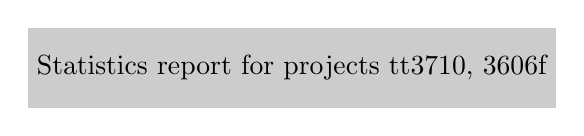
\begin{tikzpicture}
  \node [header] {
    Statistics report for projects tt3710, 3606f
  };
\end{tikzpicture}


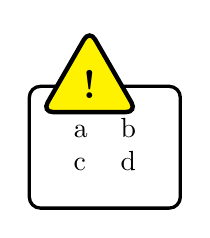
\begin{tikzpicture}
  \node [part1] (box){%
    \begin{tabular}{ll}
      a & b \\
      c & d 
    \end{tabular}
  };
  \node[title1, right = 10pt] at (box.north west) {\textbf{\Large!}};
\end{tikzpicture}%

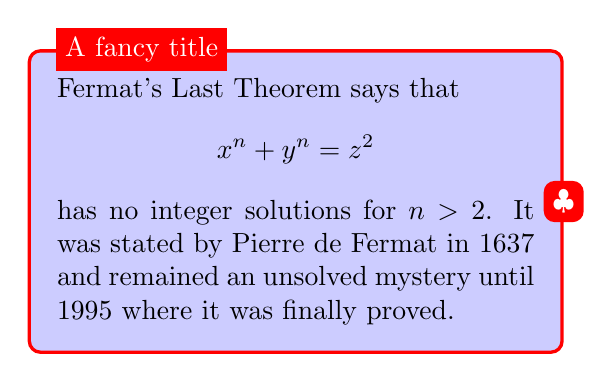
\begin{tikzpicture}%
  \node [part2] (box){%
    \begin{minipage}{0.50\textwidth}
      Fermat's Last Theorem says that
        $$
          x^n + y^n = z^2
        $$
      has no integer solutions for $n>2$. It was stated by
      Pierre de Fermat in 1637 and remained an unsolved mystery
      until 1995 where it was finally proved.
    \end{minipage}
  };
  \node[title2, right=10pt] at (box.north west) {A fancy title};
  \node[title2, rounded corners] at (box.east) {$\clubsuit$};
\end{tikzpicture}%


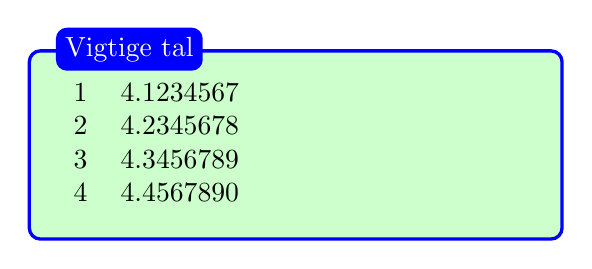
\begin{tikzpicture}%
  \node [part3] (box){%
    \begin{minipage}{0.50\textwidth}
      \begin{tabular}{ll}
         1 & 4.1234567 \\
         2 & 4.2345678 \\
         3 & 4.3456789 \\
         4 & 4.4567890 \\
      \end{tabular}
    \end{minipage}
  };
  \node[title3, right=10pt] at (box.north west) {Vigtige tal};
\end{tikzpicture}%


\end{document}
